\subsection{The multi-VoF methodology and the no-coalescence algorithm}
Objectives 
\begin{itemize}
    \item Presents the bibliography. 
    \item Introduce mani's algorithm
    \item explain step by step the algorithm
\end{itemize}


The key feature of numerical simulations is the use of a whole new algorithm which prevent numerical coalesce of droplets to occur.
First, the reader can find the described source code at \href{https://basilisk.fr/sandbox/fintzin/no-coalesce.h}{no-coalesce.h}. 
In the following we describe the global ideas and principles, then we dive into a step by step explanation of the algorithm. 
But first some worlds on the already existing algorithm is in order.

In previous studies several methods have been used to avoid coalescence. 
The first one is to increase artificially the surface tension coefficient locally such as it is done in \citet{hidman2023assessing}.
When using a level set method to track the  phase indicator function some authors developed a multiple marker level-set method to prevent coalesence, see \citet{balcazar2015multiple}. 
Similarly, for VOF tracer some author used a multi-vof approach. 
In a recent study \citet{zhang2021direct} used one VOF tracer per bubble in his simulation which prevent coalesence and allows to track bubbles independently. 
However, this approach is quite expensive as it requires solving \ref{eq:dt_alpha} for each drop. 
Instead, we adopt the methodology of \citet{karnakov2022computing} which consider a constant number of VOF tracer with respect to the number of dorplets. \JL{pr moi le nombre de Traceur VoF change aucours du temps ? par ailleurs Karnakov utilise une couleur (un champs VoF) par goutte ? non ?}
We then adoped another methodology to track bubbles independently that we adapted inside the \texttt{Basilisk} code. 

The adaptation of \citet{karnakov2022computing} within the basilisk code has been carried out by \citet{mani2021numerical} \JL{on ne peut pas vraiment dire que Mani a adapte l'algo de Karnakov. Deja car ila soutenu avant meme que cette algo soit publie et d'autre part les méthodos semblent bien differentes. En particulier, a ma connaissance le no-coalescence est unique chez nous.}, which developed an algorithm to prevents the adjacent droplets to have similar VOF tracers using the least VOF tracer as possible by allowing different drops to be included within the same VOF tracer.
Specifically we define $N(t)$ VOF tracer labeled as $\alpha_d^i$ for $i =0,\ldots,N$ where $N(t)$ is dependent on time since it is function of the particles positions.  
The only requirement is that the adjacent droplets at a given time $t$, have different VOF tracer to prevent coalescence. 


\begin{figure}[h!]
    \centering
    % \begin{tikzpicture}[scale=0.1,
    %     node distance = 4mm and 6mm,
    %   start chain = going below,
    %   base/.style = {draw, thick, fill=gray!10, align=center, 
    %                  inner xsep=2mm, inner ysep=2mm},
    %   rect/.style = {base},
    %   elli/.style = {ellipse, base},
    %   circ/.style = {circle, fill=graye!10, minimum size=12pt},
    %   diam/.style = {diamond, base, aspect=1.5},
    %   line/.style = {draw, rounded corners, -Stealth, semithick},
    % ]
    % % Place nodes
    % \begin{scope}[nodes = {on chain, join=by line}]
    % \node [rect, rounded corners=10pt] (step1) {start};
    % \node [rect] (step2) {(1) Apply tag function \\ on vof field $\alpha_d^i$};
    % \node [base] (step3) {(2) Check for any adjacent drops \\ that have the same $\alpha_d^i$};
    % \node [rect] (step5) {(3) Change drops vof tracers for all\\ adjacent drops.};
    % \node [diam] (step7) {$i < N(t)$};
    % \node [rect, rounded corners=10pt] (step8) {stop};
    % \end{scope}
    % % \node [rect, left=of step3] (step9) {$i = i+1$};
    % % Draw edges
    % % \path[line] (step7) -| (step9);
    % % \path[line] (step9) |- (step2);
    % %
    % \path       (step7) -- node [right,near start]{False}    (step8);
    % \node [right=of step5] {
        % };
        % \end{tikzpicture}
    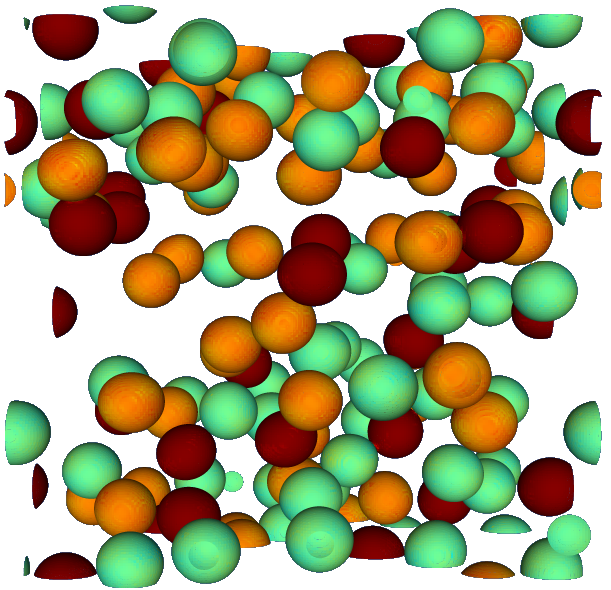
\includegraphics[width = 0.6\textwidth]{image/VOF2.png}
    \caption{
    %     Simplified flowchar of the \texttt{no-coalescence.h} algorithm.
    % $\{\alpha_d^i;i\in\mathbb{N}^{*+}\}$ represent the list of VOF tracer currently used. 
    % $N(t)$ is the total number of tracer at time $t$. 
    (b) Interface of the droplets colored by the value of $\alpha_d^i$ at $t_g =100$.
    }
    \label{fig:diagram}
\end{figure}


The simplified workflow of the algorithm follows these three steps : 
\begin{enumerate}
    \item We first identify the different topologies, i.e. the droplets, within a single tracer $\alpha_d^i$. 
    This is done by using another Basilisk feature which assign to a scalar field a different value to each topological object such as a drop (see \href{http://basilisk.fr/src/tag.h}{tag.h})\todo{biblio ?}
    \item Then we identify the droplets/tag which are different and too close to one another.
    The distance criterion is fixed to a cube of 5 mesh cells length.  
    \item Lastly we assign a new VOF tracer for each required droplets among the VOF tracer that are not already adjacent to the droplets. 
    If no VOF tracer is available we create a new one for the droplets.
    \todo{Maybe more details ?}
\end{enumerate}
This algorithm is executed at each simulation time step. 
Besides having $N$ VOF tracer require some modifications to the previously mentioned governing equations. 
Especially, instead of solving \ref{eq:dt_alpha}  we solve $N$ transport equation for each $\alpha_d^i$\todo{Is it true ?}.
But also, we compute the surface tension force as the sum of the contribution from each VOF tracer, namely, 
\begin{equation}
    \textbf{f}_\sigma \delta(\textbf{x}-\textbf{x}_I)
    = \sum_{i=0}^{N(t)} \sigma \kappa \nablab \alpha_d^i
\end{equation} 
where $\kappa_i$ is the approximate curvature of $\alpha_d^i$. 
In the 2D simulations (not presented here) we do not used more than 4 VOF tracers for hundreds of droplets during a simulation. 
This is a consequence  of the four color map theorem derived from topological arguments.
In the three-dimensional were we simulated hundreds of droplets we observed the creation of $6$ VOF tracer in the long run of the simulations \JL{aurais tu une evolution en fonction du temps du nombre de traceur VoF en fonction de la fraction volumique. Je pense que c'est un element interessant.}.
A picture of the colored VOF is shown \ref{fig:diagram} (b) where only 3 VOF tracer is needed.
Indeed, the four color map theorem isn't valid anymore therefore the increase of VOF tracer isn't surprising anymore. 

Overall, we used an optimized multi-VOF method which allows us to compute massive DNS with approximately $6$ VOF tracers. 





